% questions.tex —— 1995 年·上海卷·文史类 · 题目内容片段（无答案）
% 由 tools/generate_projects.py 依来源总账自 1995/1995_数学真题_上海文_试题.md 生成，勿手改（改源 MD 后重跑）


来源题签：“1995 年全国普通高等学校招生统一考试·上海数学试卷（文史类）”。

\begin{gktip}
来源说明：固定来源 PDF 共 7 页，扫描页 1–3 为题面，扫描页 4–7 附卷内「数学试卷答案及评分标准」。来源字节与考试身份已绑定；出版者、版次及答案是否为官方版本未核实，以下答案均注明为“卷内所载”，不冒称官方答案。全卷 25 题、满分 150 分：选择题 1–8（每题 3 分），填空题 9–20（共 48 分），解答题 21–25（共 78 分）。$A_1/B_1$ 组选做第 18–20 题，$A_2/B_2$ 组选做第 21–22 题；各组不得混做，按原卷规则计分。

图形均按原卷关系矢量重绘，不按扫描尺寸测绘。
\end{gktip}

\gkpart{一、选择题（1—8，每题 3 分）}

本大题满分 24 分。本大题共有 8 题，每题给出代号为 A、B、C、D 的四个结论，其中有且只有一个结论是正确的，必须把正确结论的代号写在题后的圆括号内，选对得 3 分，不选、选错或者选出的代号超过一个（不论是否都写在圆括号内），一律得零分。

\begin{question}
\gkti{1}$y=\sin^2x$ 是\mbox{（　　）}

（A）最小正周期为 $2\pi$ 的偶函数　（B）最小正周期为 $2\pi$ 的奇函数

（C）最小正周期为 $\pi$ 的偶函数　（D）最小正周期为 $\pi$ 的奇函数

\end{question}
\begin{question}
\gkti{2}如果 $P=\{x\mid(x-1)(2x-5)<0\}$，$Q=\{x\mid0<x<10\}$，那么\mbox{（　　）}

\begin{gkopts}(2)
\task （A）$P\cap Q=\varnothing$
\task （B）$P\subset Q$
\task （C）$P\supset Q$
\task （D）$P\cup Q=\mathbb R$
\end{gkopts}

\end{question}
\begin{question}
\gkti{3}方程 $\tan\left(2x+\dfrac\pi3\right)=\dfrac{\sqrt3}{3}$ 在区间 $[0,2\pi)$ 上解的个数是\mbox{（　　）}

\begin{gkopts}(4)
\task （A）5
\task （B）4
\task （C）3
\task （D）2
\end{gkopts}

\end{question}
\begin{question}
\gkti{4}设棱锥的底面面积是 $8\,\mathrm{cm}^2$，那么这个棱锥的中截面（过棱锥高的中点且平行于底面的截面）的面积是\mbox{（　　）}

\begin{gkopts}(2)
\task （A）$4\,\mathrm{cm}^2$
\task （B）$2\sqrt2\,\mathrm{cm}^2$
\task （C）$2\,\mathrm{cm}^2$
\task （D）$\sqrt2\,\mathrm{cm}^2$
\end{gkopts}

\end{question}
\begin{question}
\gkti{5}“$ab<0$”是“方程 $ax^2+by^2=c$ 表示双曲线”的\mbox{（　　）}

（A）必要条件但不是充分条件　（B）充分条件但不是必要条件

（C）充分必要条件　（D）既不是充分条件又不是必要条件

\Needspace{0.4\textheight}
\end{question}
\begin{question}
\gkti{6}当 $a\ne0$ 时，函数 $y=ax+b$ 和 $y=b^{ax}$ 的图象只可能是\mbox{（　　）}
\nopagebreak[4]
\begin{center}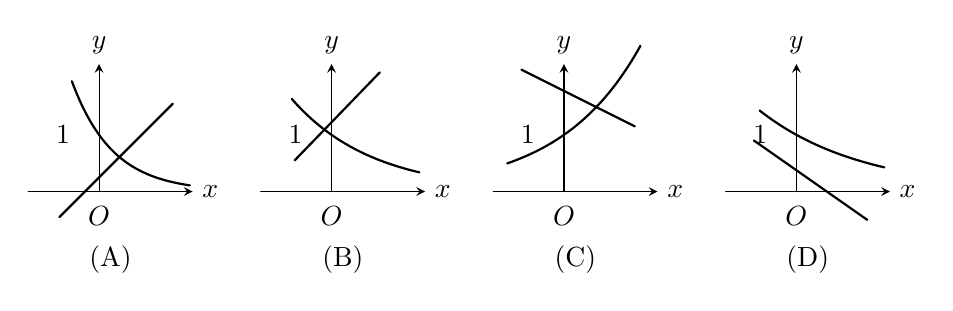
\begin{tikzpicture}[>=stealth,scale=0.72,line cap=round,line join=round]
\foreach \x/\name in {0/A,4.1/B,8.2/C,12.3/D}{
  \begin{scope}[shift={(\x,0)}]
    \draw[->] (-1.25,0)--(1.65,0) node[right] {$x$};
    \draw[->] (0,0)--(0,2.25) node[above] {$y$};
    \node[left=7pt] at (0,1) {$1$};
    \node[below=2pt] at (0,0) {$O$};
    \node at (0.2,-1.2) {(\name)};
  \end{scope}
}
% A: a>0 and 0<b<1; both curves use the same a,b.
\begin{scope}[shift={(0,0)}]
  \draw[thick,domain=-0.48:1.6,samples=80] plot (\x,{0.25^\x});
  \draw[thick] (-0.7,-0.45)--(1.3,1.55);
\end{scope}
% Distractor sketches retain the qualitative alternatives printed in the source.
\begin{scope}[shift={(4.1,0)}]
  \draw[thick,domain=-0.7:1.55,samples=80] plot (\x,{exp(-0.7*\x)});
  \draw[thick] (-0.65,0.55)--(0.85,2.10);
\end{scope}
\begin{scope}[shift={(8.2,0)}]
  \draw[thick,domain=-1.0:1.35,samples=80] plot (\x,{exp(0.7*\x)});
  \draw[thick] (-0.75,2.15)--(1.25,1.15);
\end{scope}
\begin{scope}[shift={(12.3,0)}]
  \draw[thick,domain=-0.65:1.55,samples=80] plot (\x,{exp(-0.55*\x)});
  \draw[thick] (-0.75,0.90)--(1.25,-0.50);
\end{scope}
\end{tikzpicture}
\end{center}
\nopagebreak[4]
\end{question}
\begin{question}
\gkti{7}当 $0<a<b<1$ 时，下列不等式中正确的是\mbox{（　　）}

（A）$(1-a)^{1/b}>(1-a)^b$

（B）$(1+a)^a>(1+b)^b$

（C）$(1-a)^b>(1-a)^{b/2}$

（D）$(1-a)^a>(1-b)^b$

\end{question}
\begin{question}
\gkti{8}下列四个命题中的真命题是\mbox{（　　）}

（A）经过定点 $P_0(x_0,y_0)$ 的直线都可以用方程 $y-y_0=k(x-x_0)$ 表示。

（B）经过任意两个不同的点 $P_1(x_1,y_1)$、$P_2(x_2,y_2)$ 的直线都可以用方程 $(y-y_1)(x_2-x_1)=(x-x_1)(y_2-y_1)$ 表示。

（C）不经过原点的直线都可以用方程 $\dfrac xa+\dfrac yb=1$ 表示。

（D）经过定点 $A(0,b)$ 的直线都可以用方程 $y=kx+b$ 表示。

\end{question}
\gkpart{二、填空题（9—20，共 48 分）}

本大题共有 12 题，只要求直接填写结果，每个空格填对得 4 分，否则一律得零分。

\begin{question}
\gkti{9}不等式 $\dfrac{2x-1}{x+3}>1$ 的解是 \gkblank{}。

\end{question}
\begin{question}
\gkti{10}双曲线 $\dfrac{x^2}{2}-\dfrac{8y^2}{9}=8$ 的渐近线方程是 \gkblank{}。

\end{question}
\begin{question}
\gkti{11}1992 年底世界人口达到 54.8 亿，若人口的年平均增长率为 $x\%$，2000 年底世界人口数为 $y$（亿），那么 $y$ 与 $x$ 的函数关系式是 \gkblank{}。

\end{question}
\begin{question}
\gkti{12}已知 $\log_3x=-\dfrac1{\log_2 3}$，那么 $x+x^2+x^3+\cdots+x^n+\cdots=$ \gkblank{}。

\end{question}
\begin{question}
\gkti{13}若 $(x+1)^n=x^n+\cdots+ax^3+bx^2+\cdots+1$（$n\in\mathbb N$），且 $a:b=3:1$，那么 $n=$ \gkblank{}。

\end{question}
\begin{question}
\gkti{14}到点 $A(-1,0)$ 和直线 $x=3$ 距离相等的点的轨迹方程是 \gkblank{}。

\end{question}
\begin{question}
\gkti{15}函数 $y=3x^2+1\;(x\le0)$ 的反函数是 $y=$ \gkblank{}。

\end{question}
\begin{question}
\gkti{16}函数 $y=\lg\sqrt{10^x-2}$ 的定义域是 \gkblank{}。

\end{question}
\begin{question}
\gkti{17}函数 $y=\sin\dfrac x2+\cos\dfrac x2$ 在 $(-2\pi,2\pi)$ 内的递增区间是 \gkblank{}。

\end{question}
\gksubpart{选做题：$A_1$组与$B_1$组二选一}

考生可以从下列两组（$A_1$组和$B_1$组）中选做一组试题，其中 $A_1$组适合非试点校考生，$B_1$组适合试点校考生。

\begin{question}
\gkti{18}

$A_1$组：若 $\displaystyle\lim_{n\to\infty}\left[1+(r+1)^n\right]=1$，则 $r$ 的取值范围是 \gkblank{}。

$B_1$组：$\displaystyle\lim_{n\to\infty}\left(1+\dfrac1n\right)^{n-2}=$ \gkblank{}。

\end{question}
\begin{question}
\gkti{19}

$A_1$组：从 6 台原装计算机和 5 台组装计算机中任意选取 5 台，其中至少有原装与组装计算机各 2 台，则不同的选取法有 \gkblank{} 种。（结果用数值表示）

$B_1$组：从 6 台原装计算机和 5 台组装计算机中任意选取 5 台，其中至少有原装与组装计算机各 2 台的概率是 \gkblank{}。

\end{question}
\begin{question}
\gkti{20}

$A_1$组：把圆心角为 $216^\circ$、半径为 5 分米的扇形铁皮焊成一个圆锥形容器（不计焊缝），那么容器的容积是 \gkblank{} 立方分米。（结果保留两位小数）

$B_1$组：某工程由下列工序组成：工序 $a$ 无紧前工序；$b,c$ 的紧前工序均为 $a$；$d$ 的紧前工序为 $b$；$e$ 的紧前工序为 $c,d$。工时数（天）分别为 $a:2,b:3,c:5,d:6,e:3$。那么工程总时数是 \gkblank{} 天。

\end{question}
\gkpart{三、解答题（21—25，共 78 分）}

本大题共有 5 题，解下列各题必须写出必要的步骤。

\gksubpart{选做题：$A_2$组与$B_2$组二选一}

考生可以从下列两组（$A_2$组和$B_2$组）中选做一组试题，其中 $A_2$组适合非试点校考生，$B_2$组适合试点校考生。

\Needspace{0.4\textheight}
\begin{question}
\gkti{21}

$A_2$组（本题满分 12 分）：已知 $\tan\left(\dfrac\pi4+\theta\right)=3$，求 $\sin2\theta-2\cos^2\theta$ 的值。

$B_2$组（本题满分 12 分，共 2 小题，第 1 小题满分 4 分，第 2 小题满分 8 分）：如图，在空间直角坐标系中，$BC=2$，原点 $O$ 是 $BC$ 的中点，点 $A$ 的坐标是 $\left(\dfrac{\sqrt3}{2},\dfrac12,0\right)$，点 $D$ 在平面 $yoz$ 上，且 $\angle BDC=90^\circ$，$\angle DCB=30^\circ$。
\nopagebreak[4]
\begin{center}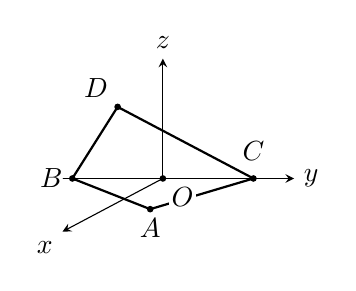
\begin{tikzpicture}[
  x={(-0.85cm,-0.45cm)}, y={(1.15cm,0cm)}, z={(0cm,1.05cm)},
  >=stealth,scale=1.0,line cap=round,line join=round]
  \coordinate (O) at (0,0,0);
  \coordinate (B) at (0,-1,0);
  \coordinate (C) at (0,1,0);
  \coordinate (A) at ({sqrt(3)/2},0.5,0);
  \coordinate (D) at (0,-0.5,{sqrt(3)/2});
  \draw[->] (O)--(1.5,0,0) node[below left] {$x$};
  \draw[->] (0,-1.1,0)--(0,1.45,0) node[right] {$y$};
  \draw[->] (O)--(0,0,1.45) node[above] {$z$};
  \draw[thick] (B)--(D)--(C)--(A)--cycle;
  \fill (O) circle (1.2pt) node[fill=white,inner sep=1pt,below right=2pt] {$O$};
  \fill (A) circle (1.2pt) node[below] {$A$};
  \fill (B) circle (1.2pt) node[left] {$B$};
  \fill (C) circle (1.2pt) node[above=3pt] {$C$};
  \fill (D) circle (1.2pt) node[above left] {$D$};
\end{tikzpicture}
\end{center}
\nopagebreak[4]
（1）求向量 $\overrightarrow{OD}$ 的坐标；（2）设向量 $\overrightarrow{AD}$ 和 $\overrightarrow{BC}$ 的夹角为 $\theta$，求 $\cos\theta$ 的值。

\end{question}
\gksubpart{共通题}

\begin{question}
\gkti{22}

$A_2$组（本题满分 14 分）：已知复数 $z_1,z_2$ 满足 $|z_1|=|z_2|=1$，且 $z_1+z_2=i$，求 $z_1,z_2$ 的值。

$B_2$组（本题满分 14 分，共 2 小题，第 1 小题满分 7 分，第 2 小题满分 7 分）：设 $y=f(x)$ 是二次函数，方程 $f(x)=0$ 有两个相等的实根，且 $f'(x)=2x+2$。（1）求 $y=f(x)$ 的表达式；（2）求 $y=f(x)$ 的图象与两坐标轴所围成图形的面积。

\Needspace{0.4\textheight}
\end{question}
\begin{question}
\gkti{23}（本题满分 16 分，共 2 小题，第 1 小题满分 9 分，第 2 小题满分 7 分。）如图，四棱锥 $P\text{-}ABCD$ 中，底面是一个矩形，$AB=3$，$AD=1$，又 $PA\perp AB$，$PA=4$，$\angle PAD=60^\circ$。（1）求四棱锥 $P\text{-}ABCD$ 的体积；（2）求二面角 $P\text{-}BC\text{-}D$ 的大小（用反三角函数表示）。
\nopagebreak[4]
\begin{center}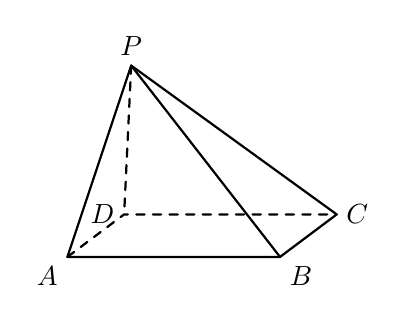
\begin{tikzpicture}[>=stealth,scale=0.9,line cap=round,line join=round]
  \coordinate (A) at (0,0);
  \coordinate (B) at (3,0);
  \coordinate (D) at (0.8,0.6);
  \coordinate (C) at (3.8,0.6);
  \coordinate (P) at (0.9,2.7);
  \draw[thick] (A)--(B)--(C)--(P)--cycle;
  \draw[thick] (P)--(B);
  \draw[thick,dashed] (A)--(D)--(C);
  \draw[thick,dashed] (P)--(D);
  \node[below left] at (A) {$A$};
  \node[below right] at (B) {$B$};
  \node[right] at (C) {$C$};
  \node[left] at (D) {$D$};
  \node[above] at (P) {$P$};
\end{tikzpicture}
\end{center}
\nopagebreak[4]
\end{question}
\begin{question}
\gkti{24}（本题满分 18 分，共 2 个小题，第 1 小题满分 6 分，第 2 小题满分 12 分。）设椭圆的方程为 $\dfrac{x^2}{m^2}+\dfrac{y^2}{n^2}=1$（$m,n>0$），过原点且倾角为 $\theta$ 和 $\pi-\theta$（$0<\theta<\dfrac\pi2$）的两条直线分别交椭圆于 $A,C$ 和 $B,D$ 四点。（1）用 $\theta,m,n$ 表示四边形 $ABCD$ 的面积 $S$；（2）若 $m,n$ 为定值，当 $\theta$ 在 $(0,\dfrac\pi4]$ 上变化时，求 $S$ 的最大值 $u$。

\end{question}
\begin{question}
\gkti{25}（本题满分 18 分，共 3 个小题，第 1 小题满分 4 分，第 2 小题满分 6 分，第 3 小题满分 8 分。）已知二次函数 $y=f(x)$ 在 $x=\dfrac{t+2}{2}$ 处取得最小值 $-\dfrac{t^2}{4}$（$t\ne0$），$f(1)=0$。（1）求 $y=f(x)$ 的表达式；（2）若任意实数 $x$ 都满足等式 $f(x)g(x)+mx+n=x^3$（$g(x)$ 为多项式），试用 $t$ 表示 $m$ 和 $n$；（3）设 $t=-3$，圆 $C_k$ 的方程为 $(x-mq^k)^2+(y-nq^k)^2=r_k^2$（$0<q<1,r_k>0$），圆 $C_k$ 与 $x$ 轴相切，圆 $C_k$ 与 $C_{k+1}$ 外切（$k=0,1,2,\ldots$），记 $S$ 为所有这些圆的面积之和，求 $q,S$ 的值。

\end{question}